\hthree{Klassisches Projektmanagement}

\hfour{Grundlegendes}

Klassisches Projektmanagement zeichnet sich dadurch aus, dass zu Beginn des Projekts ein starrer Endzustand definiert wird, welcher durch viele Anforderungen belegt wird. Außerdem wird sehr schon im Vorhinein sehr viel in die detaillierte Planung von Prozessen und Zeitmanagement gesteckt. Zum Ende hin wird aber ein Zeitpuffer gelassen um auf mögliche Änderungen oder Verzögerungen vorbereitet zu sein und diese so abwickeln zu können, dass das Projekt trotzdem zeitgerecht fertiggestellt werden kann. Klassisches Projektmanagement hängt also vom Anfang bis zum Ende zusammen und greift ineinander. 

Somit kann gesagt werden, dass klassisches Projektmanagement eine hohe Planungssicherheit für das Unternehmen bietet. Jedoch ist die Planung zu Beginn im Bereich des Geldes oder der Zeit immer weniger wichtig wurde, da die Planung meistens nicht eingehalten werden konnte. Im Jahr 2015 wurde eine Studie durchgeführt, welche bestätigte, dass 71\% aller Projekte gar nicht, oder nur zu einem gewissen Teil fertig gestellt werden konnten. Das sagt nicht, dass klassisches Projektmanagement schlecht, oder nicht mehr zeitgemäß ist, sondern, dass sicher der Projektmanager im Vorhinein gut überlegen muss, welches Managementsystem am Besten für das Projekt geeignet ist.  \cite{Projectman.}

\hfour{Anwendungsgebiete}

Klassisches Projektmanagement wird in Projekten verwendet, bei denen man weiß, dass mit wenigen Veränderungen zu rechnen ist. Es kann also von Beginn an gut und verlässlich in den Bereichen Personal, Kosten und Terminen geplant werden und es wird so eine hohe Planungssicherheit mitgebracht. Veränderungen in den vorher genannten Faktoren sind dann aber meistens mit hohen Kosten verbunden und werden so gut es geht vermieden.

Es empfiehlt sich Klassisches Projektmanagement zum Beispiel bei Projekten zu verwenden, welche in der Vergangenheit schon einmal durchgeführt wurden. Es gibt als schon Vorerfahrungen, welche in die fixe Planung des Projekts mit einfließen werden. Zusammengefasst kann aber gesagt werden, dass im Vorhinein viel Zeit in das Ausprobieren von unterschiedlichen Managementsystemen gesteckt werden soll, damit das am ehesten passende verwendet wird. \cite{Projectman.}

\hfour{"PRINCE2"}

\hfive{Allgemeines}

"PRINCE2" ist auf der Welt die am häufigst verwendete Methode für klassisches Projektmanagement. "PRINCE" steht in diesem Fall für "Projects in Controlled Environments" und ist als großbritannischer Regierungsstandard für Projekte in der Informatik entwickelt worden. Jedoch wurde die Methode auch immer häufiger auch außerhalb der Informatik verwendet und wurde 1996 mit dem Namen "PRINCE2" als Methode für Projektmanagement im Allgemeinen vorgestellt.

"PRINCE2" festigte sich schnell als Standard für Projektmanagement in Großbritannien und und über 50 anderen Ländern der Welt. Durch eine starke Festigung im Projektmanagement wird die Methode auch stetig weiterentwickelt und überarbeitet. Außerdem wurde auch eine sogenannte "Hybridmethode", also eine Mischform aus klassischem und agilem Projektmanagement entwickelt. Diese trägt den Namen\\ "PRINCE2Agile". \cite{Projectman.}

\hfive{Funktionsweise}

"PRINCE2" kann in Sieben Prozesse unterteilt und aufgespalten werden.

\begin{itemize}
    \item Vorbereiten des Projekts
    \item Lenken des Projekts
    \item Initiieren des Projekts
    \item Steuern einer Phase
    \item Managen der Produktlieferung
    \item Managen des Phasenübergangs
    \item Abschließen des Projekts
\end{itemize}

\begin{figure}[H]
    \centering
    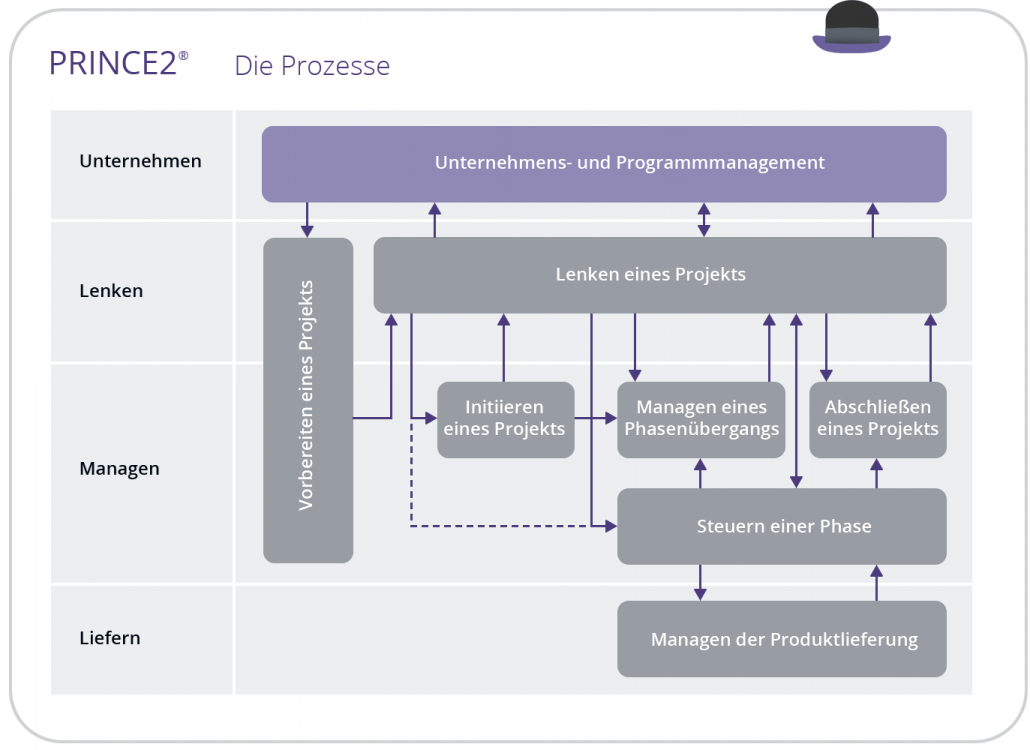
\includegraphics[width=\textwidth]{media/ProjectManagement/Prince2.png}
    \caption{Prozesse in "PRINCE2" \cite{Prince2}}
\end{figure}

\underline{Vorbereiten eines Projekts}

In dieser Phase wird sich darüber Gedanken gemacht, ob das Projekt überhaupt einen Nutzen hat und durchführbar ist. Dieser Prozess muss von einer höheren Instanz (Geschäftsführer*in oder ähnliche Funktion). Außerdem werden die wichtigen Rollen im Zuge des Projekts definiert. Dazu gehören zum Beispiel die Auftraggeber*in oder die Projektmanager*in. Weiters werden Erfahrungsberichte von vorherigen Projekten hergenommen und in die Plaung miteinbezogen und die finalen Rollen im Projektteam werden fixiert. Zum Abschluss muss die Projektmanager*in seine/ihre Planung mit einer Empfehlung auf Auflehnung oder Durchführung des Projekts dem \textbf{Lenkungsausschuss} übergeben. Es wird sofort Phase Zwei eingeleitet. \cite{Prince2}

\pagebreak
\underline{Lenken eines Projekts}

In diesem Prozess kommt der sogenannte \textbf{Lenkungsausschuss} zum Einsatz. Dieser übernimmt die Lenkung des Gesamtprojekts, während der Projektmanager die reinen Managementtätigkeiten übernimmt. Im Optimalfall kommt der \textbf{Lenkungsausschuss} nur zwischen Phasen eines Projekts zum Einsatz und hält sich ansonsten im Hintergrund. Sollte jedoch eine im Vorhinein festgelegte Puffergrenze überschritten werden greift der \textbf{Lenkungsausschuss} ebenfalls ein. Weiters übernimmt der Lenkungsausschuss die gesamte Kommunikation mit den beteiligten des Projekts (Stakeholdern).

Dieser Prozess ist nun für die Interaktion mit unterschiedlichen Prozessen, wie zum Beispiel die Freigabe für etwas, zuständig.

\underline{Initiieren des Projekts}

\underline{TODO: Weiterschrieben}
